\documentclass[letterpaper,11pt]{article}
\usepackage{array}
\usepackage{graphicx}
\usepackage{subcaption}
\usepackage{pdfpages}
\usepackage{changepage}
\usepackage{color}
\usepackage[hyphens,spaces,obeyspaces]{url}
\usepackage[colorlinks=true,urlcolor=blue,citecolor=black]{hyperref}
\usepackage[title]{appendix}
\usepackage{float}
\usepackage{listings}
\usepackage{amsmath}
\usepackage{cleveref}
\usepackage{tikz}
\usepackage{arydshln}
\usetikzlibrary{shapes,arrows}
\usetikzlibrary{positioning}
\usepackage[margin=1.5in]{geometry}
\linespread{1.1}
\setlength{\parindent}{30pt}
\setlength{\emergencystretch}{3em}
\setlength\dashlinedash{0.2pt}
\setlength\dashlinegap{1.5pt}
\tikzstyle{arrow} = [thick,->,>=stealth]
\tikzstyle{utxo} = [
    rectangle, minimum width=3.8cm, minimum height=4cm, text centered, text width=3.8cm,
    scale=0.85, draw=black, font=\ttfamily]
\tikzstyle{contract} = [
    rectangle, minimum width=3.8cm, minimum height=4cm, text centered, text width=3.8cm,
    scale=0.85, draw=black, font=\ttfamily, fill=gray!5]

\title{\LARGE BAND\\
    \Large Unleashing Tokenized Economy}
\author{
        Soravis Srinawakoon\\
        \small\href{mailto:soravis@bandprotocol.com}
            {\nolinkurl{soravis@bandprotocol.com}}
    \and
        Sorawit Suriyakarn\\
        \small\href{mailto:swit@bandprotocol.com}
            {\nolinkurl{swit@bandprotocol.com}}
    }
\date{\today\\\small Draft Version 0.1.4}
\begin{document}

\maketitle

\begin{abstract}

Band Protocol is a decentralized, permissionless blockchain protocol to create tokenized marketplace and token-curated community. Band Protocol enables seamless issuance of personalized Community Token through a continuous bonding curve, a smart contract that mints and burned personalized token through a predefined mathematical function based on current circulating supply. Any entities ranging from businesses, brands and celebrities can create a loyal token-curated community with personalized tokens. Personalized Community Token is a utility token representing primary currency, subscription, discount, reward point, or any other use cases within the community as defined by the Community Manager.

Band Protocol standardizes Product Token as a way for community manager to issue products and services. It enables both tokenized real-world products as well as new digital asset creation such as rare digital collectibles and attention token.

Band Protocol enables the creation of subscription business model. Followers can stake their Community Token to a staking contract and receive regular benefits similar to normal subscription or membership. Band Protocol allows Community Manager to define their subscription tier and discount token. Discount token is a tokenized discount voucher used to reward loyal followers and incentivize active participants rather than speculators. The amount of discounts can be customized by Community Manager and in general is proportionate to the amount of total network value. Discount tokens will be an incentive for loyal followers to stake their tokens and promote the growth of the community.

Band Token is the native utility token on the delegated-proof-of-stake Band Chain. Band Token are used to secure the network, provide global liquidity to every Community Token, and act as a governance token for future protocol upgrade.

\end{abstract}

\newpage
{
\hypersetup{linkcolor=black}
\tableofcontents
}
\newpage

\section{Introduction}

\subsection{Tokenized Economy}

A typical market-based economy involves the exchange of goods and services through barter or a medium of exchange. Traditionally, buyers exchange physical coins and banknote with physical products or services offered by sellers. As technology progresses, Internet has enabled digital economy whereby goods and services are being exchanged with digital money. E-commerce experiences exponential growth as people can conveniently conduct transaction with people across the world. Centralized companies start to dominate marketplace platform and payment gateway which are key enablers of the digital economy.

Blockchain and crypto assets are giving rise to yet another revolution in the economy. Bitcoin~\cite{nakamoto}, the first cryptocurrency, becomes the first decentralized currency which enables trustless, censorship-resistant payment. Cryptocurrency such as Bitcoin allows anyone to send transaction to anyone around the world at a fraction of a cost and a fraction of time required for traditional financial institutions to conduct similar transaction. As payment and currency are being tokenized, traditional asset is slower to experience similar tokenization process. Regulation and usability are two key factors that hinder the explosive growth of asset tokenization. Asset tokenization has clear benefits:
\begin{itemize}
\item Global accessibility
\item Liquidity premium
\item Low transaction fee
\item Transparency
\item Security
\end{itemize}

Similar to how physical trade transitions to digital trade by the advancement of the Internet, the next era of commerce is the transition from centralized digital trade to decentralized token trade. Tokenized economy will become prevalent as both real-world assets and payment are being tokenized. Band Protocol enables asset tokenization and creates a standard platform for tokenized economy.
\newpage

\subsection{Token-curated Community}
Typically, economy centers around community with common shared interest. There are multiple layers of community depending on the focus. A country is one big community where everyone shares geographical border, culture, tradition, customs and beliefs. Soccer players and followers together is another community where everyone shares interest in the sport which leads to an economic activity around soccer team and players. This leads to two sides of participant in the community: buyers and sellers. While they share similar interest in the same community, they often have conflicting needs as both sides try to maximize their own utility at the expense of the other side. Soccer team would raise their ticket price as they gain more popularity while their loyal followers have to keep paying more. Conversely, followers will not go out of their way to promote their favorite artist because they have very little economic incentive to do so. Their incentives are not truly aligned.

Crypto asset becomes the answer to which community members can finally have an aligned incentive to grow the community together. A token-curated community is a community centered around a personalized Community Token whose value closely tie to the overall network value of the community. Community Token acts as a shared economic incentive for both buyers and sellers to promote the growth of the community. Band Protocol standardizes the creation of token-curated community and details how personalized Community Token's value can be derived from overall community value through staking and discount mechanism.

%Currently companies, brands and celebrities struggle to engage with their loyal customers and followers. They mostly utilize social media channels such as Facebook, Twitter, and Instagram to cultivate their community. However, it is becoming more difficult to monetize their fan base. Many celebrities try to monetize their followers by advertising products from other companies to their followers, which is not always in the best interest of the community. For example, recent Thai celebrities are facing lawsuit because they advertise non-FDA-approved cosmetics. Influencers accept payment to promote products inorganically which misleads their followers. Similarly, content distributor channel like Youtube and Spotify are taking a big cut from content provider. Newcomers find themselves much more difficult to compete for attention and create network effect, which was originally promised by these platforms.


\subsection{Use Cases}
\begin{itemize}
\item A new musician creates a new community and publishes her first album. She cultivates and rewards early adopters through her Community Token. By having skin-in-the-game token, early adopters rally behind her success and help her grow the community.
\item Bruno Mars issue Bruno Token which can be staked to receive constant discount for all future products, priority queue to purchase concert ticket, and right to access VIP zone during meet and greet session. Bruno Mars also sell rare digital cards which contain non-public photos of the band and digital artwork.
\item Established company creates a community to curate information around a company and reward active participants with community token. Similar to how Barilla encourages followers to post new recipe on Facebook Page, now active participants can receive Barilla Token to purchase Barilla products as an incentive to curate information inside Barilla community.
\end{itemize}

\subsection{BAND Architecture} \label{sec:band-architecture}

BAND architecture consists of three main layers shown in figure~\ref{fig:pyramid}:

\begin{itemize}
\item \textbf{BAND Blockchain Layer} provides backbone blockchain network to support the entire BAND ecosystem. This includes design of cryptographic algorithm for public-private key management, gas allocation, blockchain internal state representation, on-chain price oracle and native BAND Token.
\item \textbf{BAND Protocol Layer} provides standard contracts to facilitate tokenized economy by enabling creation of personalized-token-curated community, tokenized products, token subscription model, discount token, attention curation market, etc.
\item \textbf{Application Layer} is the consumer-facing application that utilize the underlying BAND blockchain and protocol and serve real-world needs. Any developers can create a solution on top of open, permissionless BAND Protocol. Campbase will be the first application built on top of BAND.
\end{itemize}

\begin{figure}[h]
    \centering
    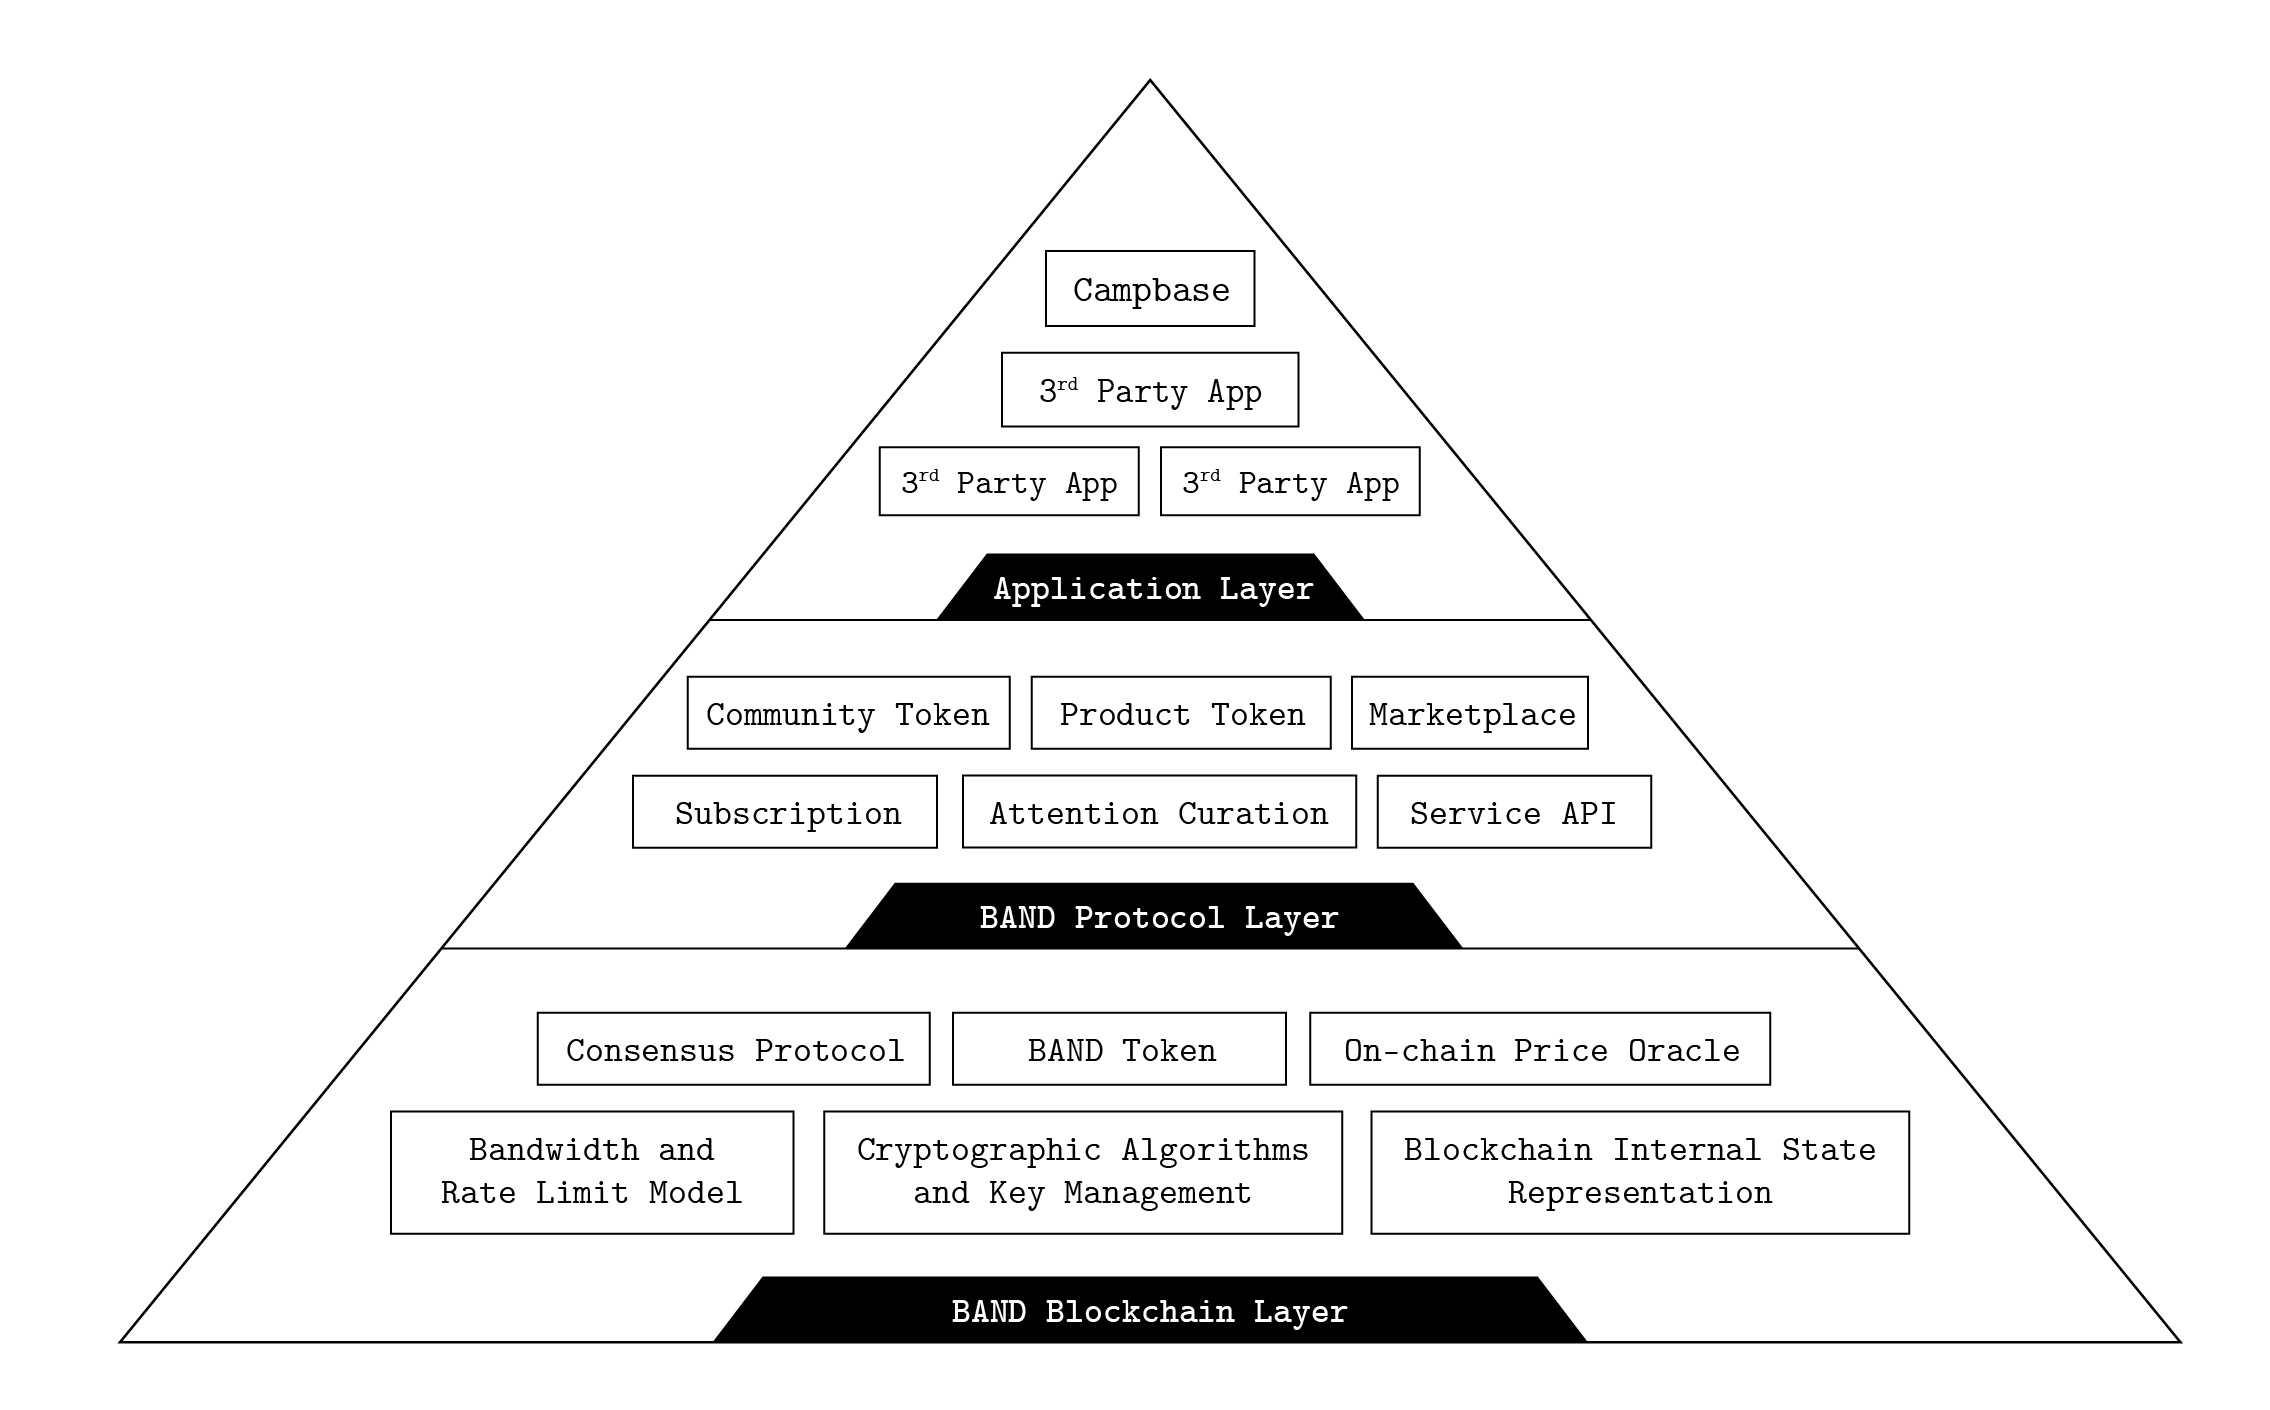
\includegraphics[width=1.05\textwidth]{figures/pyramid}
    \caption{Overview of BAND architecture}
    \label{fig:pyramid}
\end{figure}

\clearpage
\newpage

\section{Blockchain Layer} \label{sec:blockchain-layer}
This section discusses the overview of the blockchain layer in the BAND architecture. Please refer to yellow paper for full formal specification of blockchain states and transactions.

\subsection{Delegated Proof-of-Stake Protocol} \label{sec:dPOS}
BAND Protocol Layer is fundamentally independent of consensus mechanism. Tendermint, which utilizes delegated proof-of-stake, is chosen as the consensus protocol as BAND prioritizes scalability and usability over sovereign-grade security.

\subsubsection{Tendermint}
Tendermint~\cite{kwon2014tendermint} is a partially synchronous Byzantine fault tolerance consensus protocol. In BAND protocol, Tendermint is responsible for connecting the nodes and ensuring that the validators agree on a block, while BAND protocol implements Tendermint's Application BlockChain Interface (ABCI) and is responsible for maintaining the blockchain state and verifying transactions. We decide to use Tendermint in the first stage of development for several reasons:

\begin{itemize}
\setlength\itemsep{0em}
\item Tendermint is widely adopted and well recognized. It is currently used by multiple real-world blockchain systems, such as Cosmos~\cite{cosmoswhitepaper} and OmiseGo~\cite{omgtendermint}. The source code is fully open-source and has undergone public reviews.
\item Tendermint is able to handle more than 10,000 transactions per second with minimal block confirmation time~\cite{tendermint10k}.
\item Tendermint consensus protocol can quickly identify malicious actors, allowing blockchain application to quickly punish them. It is also resistant against most existing attack vectors.
\end{itemize}

\paragraph{Consensus}
In Tendermint, each node that participate in the consensus has a non-negative voting power. To produce a block, more than $\frac{2}{3}$ of the voting power must agree on the block validity. Tendermint allows ABCI to specify the voting power of each node. BAND protocol gives each node a voting power proportionally to the amount of BAND token staked by that node.

\paragraph{Validators}
Tendermint performance will degrade with more number of validators, as more validators introduce more overhead in terms of network communication and node computation. Thus, BAND protocol only allows up to certain number of active validators at any point in time, which is the top $n$ stakers by the amount of staked BAND token. All other stakers will not be able to produce blocks. To circumvent this problem, BAND protocol allows anyone to delegate their staked BAND for another party. With this, stakers can earn from BAND inflation regardless of the amount of BAND they have. Note that if the person one is staking for is acting maliciously, one loses all BAND that was delegated to the malicious person.

\subsubsection{Blockchain Parameters}
\paragraph{Block Size} There is no traditional block size limit. However, a block is limited to contain at most 10,000 transactions. Assuming average transaction size is approximately 100 Bytes, the average maximum block size is 1 Megabytes.

\paragraph{Block Time} The expected block time is 1 second. From experiment, Tendermint is able to consistently handle the workload of 10,000 transactions per second~\cite{tendermint10k}.

\paragraph{Validator Count} As discussed earlier, Tendermint gets slower as the number of validators grows. The number of validators at the genesis block is limited to 10. This number will slowly increase at a fixed rate until it reaches 100 validators over a 10-year period.

\begin{center}
\begin{tabular}{ c | c }
Year & \# of validators \\ \hline
1 & 10 \\
2 & 20 \\
3 & 30 \\
... & ... \\
10 & 100 \\
\end{tabular}
\end{center}

\paragraph{Block Reward} We set the inflation rate of 5\% per year as the reward for block validators. Because there are expectedly 31,536,000 blocks per year (1 block per second), the reward per block is $\frac{1}{6307200}$ times the current total BAND token supply.

\paragraph{Block Penalty} Tendermint protocol halts if at least $\frac{1}{3}$ of the voting power fail to accept a proposed block. To disincentivize validators from not participating, validators that have not participated in 300 blocks (5 minutes) lose 1\% of their staked BAND and automatically have all of their BAND unstaked. If a validator acts maliciously, his proposed block will be rejected by majority of the voting power. In that case, the validator lose all of his staked BAND token.

\subsection{Incentives and Fees} \label{sec:incentives-and-fees}
One of BAND protocol's main design goals is ease of usage. We carefully design the protocol to have no explicit transaction fee without introducing vulnerability to the blockchain. To achieve this goal, the transaction doesn't need to include a fee, but instead need to include a gas. The rules work as follows:

\begin{itemize}
\setlength\itemsep{0em}
\item 36,000,000 gas is created every hour, distributed to everyone proportionally to the amount BAND he is currently staking.
\item Every transaction must include exactly one gas. This means there is a hard cap of 36,000,000 transactions per hour, or 10,000 transactions per second.
\item Existing gas is invalidated every hour. At that time, everyone will be able to request a new allocation of gas for the new hour.
\end{itemize}

With this system in place, there is no need for transaction fee. It is possible, however, for a gas to be sold in secondary market for those who need more bandwidth. In the application layer, we expect application owners or community managers to provide gas for users. BAND Protocol allows a transaction to be augmented with gas by a third party without tempering with the transaction information itself.

\subsection{Cryptographic Keys}
This subsection provides a short summary of cryptographic algorithms used in BAND protocol.

\paragraph{Public-Private key pair} BAND protocol uses Ed25519~\cite{bernstein2012high} algorithm for public/private key verification.

\paragraph{Multiple Private keys} BAND protocol promotes the practice of not reusing private key to ensure pseudo-anonymity~\cite{moser2013anonymity}. BAND allows anyone to generate their single \emph{super private key} that acts as a seed to generate more private key with a nonce. A private key is simply $sha256(super\_private\_key + nonce)$. Every address on chain will have an associated nonce, so that the owner can easily generated his private key based on that nonce. Note that the nonce information is not useful to anyone that does not have the super private key.

\paragraph{Address} Similar to Bitcoin~\cite{nakamoto} and Ethereum~\cite{wood2014ethereum}, BAND protocol does not directly use public key as an address. Instead, the last 160 bits (20 bytes) of public key is used as the address. This decision is done to mitigate effect of the unlikely event that Ed25519 is compromised. It also makes the public key not revealable until there is a transaction interacting with it.

\subsection{BAND Protocol State}
BAND's blockchain state is made up of two different object types: unspent transaction output (UTXOs) and static contracts. The subsection provides a high-level overview of the two object types.

\subsubsection{Unspent Transaction Outputs (UTXOs)}
A UTXO represents an amount of tokens owned by a person in the network. BAND UTXOs are conceptually similar to Bitcoin UTXOs, with one subtle difference: there is more than one type of tokens in the network. Once a UTXO is created, its information cannot be changed, though it can be destroyed when being spent. In order to spend a UTXO as part of a transaction, the owner must prove UTXO ownership by signing the transaction with one of his private keys matching the UTXO's owner address. In this paper, a UTXO is depicted as a white rectangular box containing its information.

\subsubsection{Static Contracts}
A static contract is everything else in the blockchain that is not exclusively owned by one party (i.e. not a UTXO). A static contract always has a static address to which UTXOs or transactions in the network can refer to. Once a static contract is created, it stays forever and cannot be destroyed, though the values inside the contract may change as a result of a transaction being processed. In this paper, a static contract is depicted as a grayed rectangular containing its information.

\begin{figure}[!h]
\centering
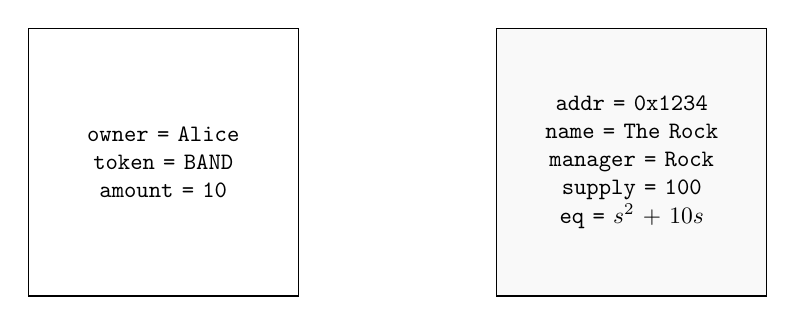
\begin{tikzpicture}[node distance=7cm]
\node (node1) [utxo] {
    owner = Alice \\
    token = BAND \\
    amount = 10
};

\node (node2) [contract,right of=node1] {
    addr = 0x1234 \\
    name = The Rock \\
    manager = Rock \\
    supply = 100 \\
    eq = $s^2 + 10s$
};
\end{tikzpicture}
\caption{Left box is a UTXO representing 10 BAND token owned by Alice. Right box is a contract representing the current state of community token ``The Rock'' living at static address {\tt 0x1234}, with Rock as the community manager, current token supply of 100 The Rock, and value-supply equation of $V(s) = s^2 + 10s$.}
\label{fig:utxo-contract-example}
\end{figure}

\subsection{On-Chain Price Oracle} \label{sec:on-chain-px-oracle}
BAND protocol is built to be aware of external off-chain price information. This allows on-chain fiat pricing in Product Token insurance contracts (\Cref{sec:product-token}), tradable UTXOs (\Cref{sec:marketplace}), and permission contracts (\Cref{sec:permission-contracts}). To achieve this goal, BAND protocol requires that every block must contain the following price information. Note that this list can be extended later as necessary.

\begin{itemize}
\setlength\itemsep{0em}
\item $P_{\mathit{BNDUSD}}$ : The volume-weighted average price of BAND token and US Dollar across all cryptocurrency exchanges.
\item $P_{\mathit{EURUSD}}$ : The conversion rate between Euro and US Dollar.
\item $P_{\mathit{GBPUSD}}$ : The conversion rate between British Pound and US Dollar.
\end{itemize}

For a block with price information to be committed, the majority of consensus participants must agree on the price values (Refer to~\cref{sec:dPOS} for consensus detail). Nodes will accept any price within 1\% error threshold. To prevent one bad price from having a direct influence on the token pricing, the protocol uses the median price among 120 consecutive blocks as one valid price data point. Given block time of one second, a single data point comes from a median price over a period of two minutes. Additionally, to prevent short-term price manipulation, on-chain price is the median among last 30 data points. Thus a price at any point is the median of price in the past one hour. Notice that with this approach, the on-chain price will not change more frequently than every two minutes. This reduces chances of transaction, which derives BAND token price based on $P_{\mathit{BNDUSD}}$, getting invalidated when the blockchain is backlogged and potentially lead to more backlogged transactions.

\begin{figure}[!ht]
 \begin{adjustwidth}{-0.5cm}{}
\begin{tabular}{c|c|c|c|c|c|c|c|c|c|c|c|c|c|c|c}
 & 1 & 2 & 3 & 4 & 5 & 6 & 7 & 8 & 9 & 10& 11& 12& 13& 14& 15\\ \hline
datapoint 1 & {\color{cyan} 32} &7 &66 &{\color{cyan} 42} &55 &67 &61 &41 &38 &1 &{\color{cyan} 27} &59 &33 &45 &21 \\
datapoint 2& 18 &52 &{\color{cyan} 62} &60 &{\color{blue} 37} &64 &75 &65 &{\color{cyan} 35} &34 &5 &3 &15 &14 &56 \\
datapoint 3& 8 &{\color{cyan} 44} &74 &29 &23 &{\color{cyan} 43} &{\color{cyan} 48} &17 &25 &51 &4 &46 &{\color{cyan} 36} &{\color{cyan} 39} &69 \\
datapoint 4& 47 &70 &12 &71 &49 &30 &13 &20 &53 &{\color{cyan} 9} &73 &{\color{cyan} 26} &54 &63 &72 \\
datapoint 5& 40 &31 &58 &19 &16 &10 &28 &{\color{cyan} 24} &22 &2 &57 &11 &50 &6 &{\color{cyan} 68} \\
\end{tabular}
\caption{Illustration of median of medians algorithm over 75 data points split into 15 groups of 5. Cyan numbers are the medians of their groups. The median of medians is shown in blue. In BAND protocol, price information for each group is collected every second over the period of 2 minutes (group size of 120). The on-chain price is the median over the most recent 30 groups.}
\end{adjustwidth}
\end{figure}

\subsection{BAND Token}
BAND token is the primary network token native to BAND Protocol. At blockchain level, an amount of BAND tokens is represented as a UTXO containing the amount and its owner's address. BAND token serves three primary functionalities.
\begin{enumerate}
\setlength\itemsep{0em}
\item Secure the network and prevent network spam through staking.
\item Act as network token to provide global liquidity to each of the Community Tokens through continuous bonding curve model.
\item Serve as a future governance token to vote on protocol upgrade as well as curating a list of future communities.
\end{enumerate}

\subsubsection{Staking}
The protocol allows network participants to stake their BAND tokens in exchange for consensus voting power (See~\cref{sec:dPOS}) and network bandwidth (See~\cref{sec:incentives-and-fees}). To stake BAND token, the owner of a BAND UTXO sends a {\tt STAKE} transaction to the network transforming the BAND UTXO into a staked BAND UTXO of the same amount. To un-stake the token, the owner sends an {\tt UNSTAKE} transaction, effective undoing the previous {\tt STAKE} transaction. Staked BAND UTXOs are different from UTXO because they cannot be spent until they get transformed back to BAND UTXOs.

\begin{figure}[!h]
\centering
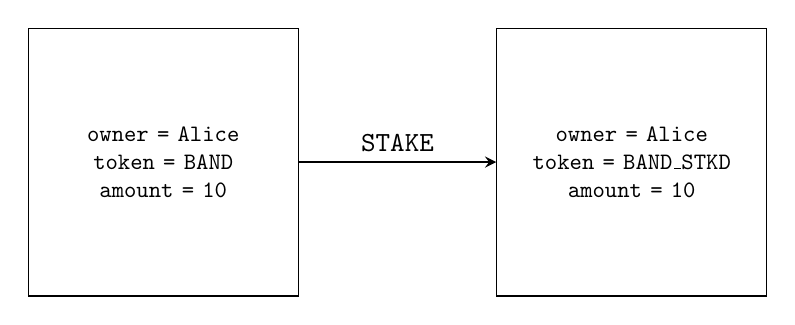
\begin{tikzpicture}[node distance=7cm]
\node (node1) [utxo] {
    owner = Alice \\
    token = BAND \\
    amount = 10
};

\node (node2) [utxo, right of=node1] {
    owner = Alice \\
    token = BAND\_STKD \\
    amount = 10
};

\draw [arrow] (node1) -- node[anchor=south] {{\tt STAKE}} (node2);
\end{tikzpicture}
\caption{An action of staking 10 BAND token by Alice}
\label{fig:utxo-stake}
\end{figure}

\subsubsection{Bonding}
BAND tokens are used as collateral to issue any Community Token through a continuous bonding curve. After Community Manager defines a bonding curve equation, anyone can buy Community Token by sending BAND token to the contract. Conversely, anyone can sell Community Token back to the contract to receive BAND Token. The buying and selling prices are algorithmically adjusted based on the Community Token's circulating supply and the bonding curve equation. Please refer to~\cref{sec:community-token} for more technical discussion regarding Community Token.

Similar to how there is a long tail of {\tt ERC20 Token}, there will be a long tail of less liquid Community Token as communities are fragmented. BAND token acts as a network token to provide global liquidity between all Community Token and thus anyone can buy, sell or switch between any Community Token with instant liquidity.

% As many communities develop on Band Protocol, there will be many specific community tokens being issued. While there will be major communities where there are many transactions to buy and sell Community Token, there will also be a long tail of community tokens with less liquidity as communities are fragmented. By bonding their community tokens to Band Token, Band Token acts as a network token that ensures instant liquidity between all community tokens.

\subsubsection{Governance and Token-Curated Registries}
Once BAND protocol is deployed and used by multiple communities, its internal logic cannot be changed easily. To upgrade, one must deploy new contract that may potentially fork the community and cause disruption among existing, working communities. Upgrade can affect security and usability of the system and therefore cannot be taken lightly. BAND Token will act as a governance token for stakeholders in every community to vote for future decentralized upgrade and governance issues. This ensures that every stakeholders will thoroughly vet new protocol upgrades and vote in favor of those that truly align with the best interest of the communities.

While initially the first set of communities will be strictly handpicked, as project moves toward complete decentralization, there will be a mechanism to maintain a registry of communities and associated Community Manager who has the right to create and maintain the community. Since there can potentially be bad actors who impersonate others, there need to be a trusted source of registry that maintains ownership right. Hence this requires a token-curated registry where BAND Token stakeholders will verify and vote to approve community creation. In order to create a community, Community Manager must submit their application along with BAND Token as a collateral, and BAND Token stakeholders must either accept or reject such application. Since the value of BAND Token tie closely to the quality of communities being developed on the protocol, stakeholders have strong incentive to maintain a high quality list of communities.

\newpage

\section{BAND Protocol}
BAND Protocol is a decentralized protocol to create tokenized marketplace and token-curated community using a set of built-in smart contracts. The protocol has been designed to maximize usability and real-world adoption of both the protocol and applications built on top. Community Managers can easily create their community and sell their tokenized products and services similar to how they would offer those products and services in the real world. Similarly, consumers can easily discover, join and participate in the communities of their interest. With open-source protocol, developers can easily create user-friendly applications on top of the protocol.

BAND Protocol aims to standardize the way community, marketplace, products and services can be offered using blockchain technology. Below is a standard set of contracts BAND Protocol offer and their interaction. More information for each contract is detailed in the subsequent sections.

\bigbreak
\begin{figure}[h]
    \centering
    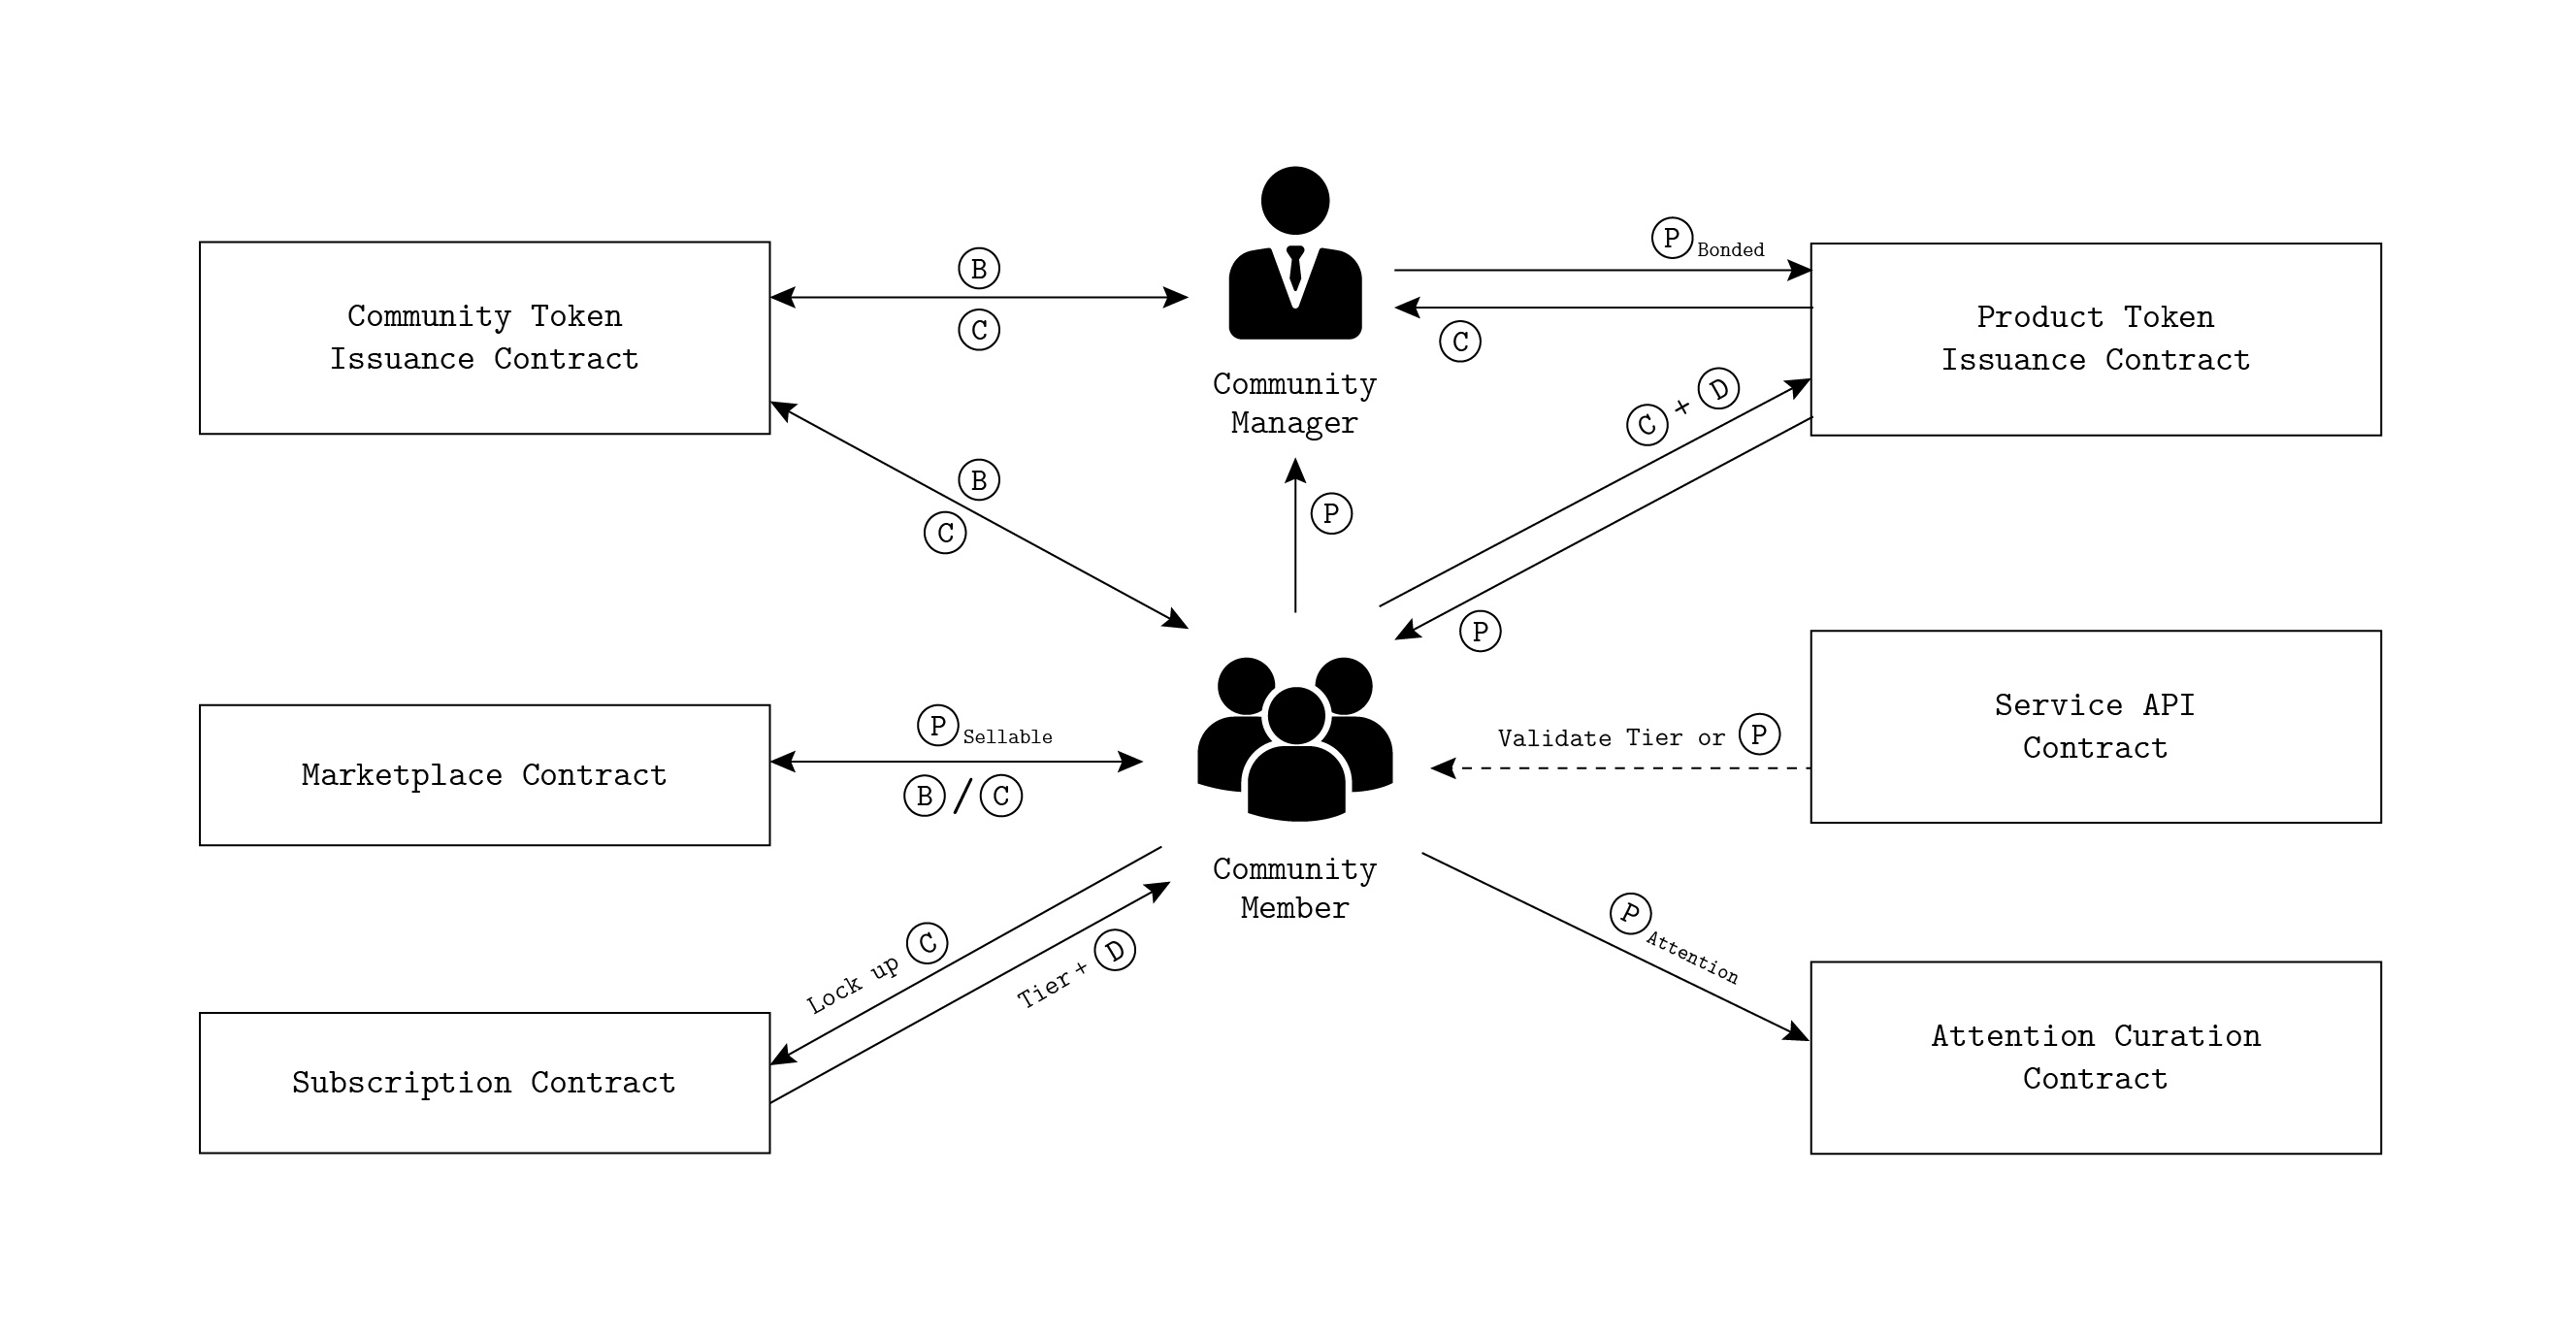
\includegraphics[width=1\textwidth]{figures/protocol}
    \caption{Overview of BAND Protocol Layer and interactions between Community Manager and community member. Arrows represent transaction and function call while circles represent cryptographic tokens. A letter inside circle represents different type of token: B for BAND Token, C for Community Token, P for Product Token, and D for Discount Token.}
    \label{fig:bandlayer}
\end{figure}

\newpage
\subsection{Community Token} \label{sec:community-token}
Community Token is a personalized token used to curate a specific community. It has three utilities within the issued community:

\begin{enumerate}
\setlength\itemsep{0em}
\item Serve as primary currency and unit of account to purchase products and services
\item Access to subscription services (e.g. unlimited music streaming, discount voucher)
\item Create personal attention curation market by voting with their tokens
\end{enumerate}
Community Token can be issued via a standard Community Token Issuance Contract with customized parameter set by the Community Manager. Once the contract is launched, anyone can purchase newly issued Community Token by bonding their BAND Token with the contract. The Community Token can then be used within the specific community. Community Token can also be sent back to the Issuance Contract to redeem back collateralized Band Token. The price is determined by predefined bonding curve function set by Community Manager which is positively correlated with total circulating supply of Community Token. Note that there is no secondary market for Community Token. There are three parameters that the creator must specify:

\begin{itemize}
\setlength\itemsep{0em}
\item Value-Supply equation
\item Maximum supply
\item Price spread
\end{itemize}

\subsubsection{Value-Supply Equation} This equation describes the relationship between the Community Token's total supply and its total value in terms of BAND token. In other words, given the current supply $s$, $V(s)$ produces the total number BAND collateralized in the Community Token Contract. Notice that by defining this value-supply equation, one can easily derive the price of Community Token at the current total supply $P(s)$ as the derivative of the value-supply equation at the specific supply value:
\bigbreak
\begin{align*}
P(s) &= \frac{d}{ds}V(s) & \text{; or in other words} \\
V(s) &= \int_{0}^{s} P(s) ds
\end{align*}

The total price of buying $x$ Community Tokens at total supply $s$ is thus $V(s+x)-V(x)$, or $\frac{V(s+x)-V(x)}{x}$ per token on average. As an example, if the Community Manager would like to have the price-supply equation $P(s) = 2s + 10$, he must specify the on-chain value-supply equation $V(s) = s^2 + 10s$. If community member would like to buy 3 tokens when the current supply is 100, they must pay $V(103)-V(100) =639$ BAND, or 213 BAND per token. Notice that this is consistent with the price-supply equation and works even when a person wants to buy non-integral amount of Community Token.

BAND protocol allows flexibility in the equation. Specifically, any equation that can be described in terms of recursive applications of common unary and binary expressions on the current total supply and constant numbers can be encoded on chain. The grammar of value-supply equation can be formalized as:
\begin{align*}
V \leftarrow
\begin{cases}
V \bigoplus V & \text{binary operation -- addition, subtraction, } \\
& \text{multiplication, division, modulus, and exponentiation} \\
\pm V & \text{unary operation -- negation, sine, and cosine} \\
s & \text{current token supply} \\
c & \text{integral constant}
\end{cases}
\end{align*}

There are three major types of curve that should be useful at the initial stage of deployment.
\paragraph{Monomial Curve} In this model, price is described as a monomial function in terms of total supply. Price of the Community Token positively correlates with its circulating supply. This encourages community curation and discourages selling. Note that this model is similar to what Bancor~\cite{bancorwhitepaper} offers. The following graph shows an example of a monomial curve with $P(s) = 2s$ and $V(s) = s^2$

\begin{center}
\begin{tikzpicture}
\draw[->] (0,0) -- (3,0) node[right] {$s$};
\draw[->] (0,0) -- (0,3) node[above] {$P(s)$};
\draw[scale=0.3,domain=0:10,smooth,variable=\x,red] plot ({\x},{\x /5});
\end{tikzpicture}
\begin{tikzpicture}
\draw[->] (0,0) -- (3,0) node[right] {$s$};
\draw[->] (0,0) -- (0,3) node[above] {$V(s)$};
\draw[scale=0.3,domain=0:10,smooth,variable=\x,blue] plot ({\x},{\x*\x / 10});
\end{tikzpicture}
\end{center}

\paragraph{Polynomial Curve} This is an upgraded version from the normal monomial curve. In this model, we remove the restriction that $P(0) = 0$ on monomial curve, allowing the Community Manager to set the base price of the token at the cost of more complicating curve. The following graph shows an example of a polynomial curve with $P(s) = 3s^2 - 2s + 100$ and $V(s) = s^3 - s^2 + 100s$

\begin{center}
\begin{tikzpicture}
\draw[->] (0,0) -- (3,0) node[right] {$s$};
\draw[->] (0,0) -- (0,3) node[above] {$P(s)$};
\draw[scale=0.3,domain=0:10,smooth,variable=\x,red] plot ({\x},{(3*\x*\x - 2 * \x + 100)/200});
\end{tikzpicture}
\begin{tikzpicture}
\draw[->] (0,0) -- (3,0) node[right] {$s$};
\draw[->] (0,0) -- (0,3) node[above] {$V(s)$};
\draw[scale=0.3,domain=0:10,smooth,variable=\x,blue] plot ({\x},{(\x*\x*\x - \x*\x + 100*\x)/200});
\end{tikzpicture}
\end{center}

\paragraph{Fixed Curve} In this model, the price simply does not correlate to the current supply. In other words, the total value is directly proportional the the current supply. This may seem silly at first glance, but it has the benefit of simplicity because the token always costs the same to buy. Community Manager may choose this pricing model and focus more on other curating aspects, such as subscription model (See~\cref{sec:subscription-model}. Community Manager can also choose to limit the maximum token supply (See~\cref{sec:max-supply}). Note that fixed price does not necessarily mean buy price equal to sell price (See~\cref{sec:px-spread}). The following graph shows a simple fixed curve with $P(s) = 1$ and $V(s) = s$.

\begin{center}
\begin{tikzpicture}
\draw[->] (0,0) -- (3,0) node[right] {$s$};
\draw[->] (0,0) -- (0,3) node[above] {$P(s)$};
\draw[scale=0.3,domain=0:10,smooth,variable=\x,red] plot ({\x},{(1});
\end{tikzpicture}
\begin{tikzpicture}
\draw[->] (0,0) -- (3,0) node[right] {$s$};
\draw[->] (0,0) -- (0,3) node[above] {$V(s)$};
\draw[scale=0.3,domain=0:10,smooth,variable=\x,blue] plot ({\x},{(\x});
\end{tikzpicture}
\end{center}

Pricing strategy can involve complex mathematical expressions, including trigonometry functions and integer modulus. BAND protocol leaves room for flexibility and innovation as crypto communities continue to experiment with new bonding curve and develop new pricing strategy.


\subsubsection{Maximum Supply} \label{sec:max-supply}
Another parameter that Community Manager can specify is the total maximum supply of Community Token. This variable prevents the total number of Community Token issued by the contract to never go beyond the given value.

\subsubsection{Price Spread} \label{sec:px-spread}
In addition to the primary bonding curve equation, Community Manager is able to enforce the buy-sell price spread on the Community Token Contract. The protocol natively allows two different flavors of price spread during contract creation.

\paragraph{Constant Spread} At any time, the price of selling 1 community token is lower than buying 1 community token by c BAND unit.
\paragraph{Rational Spread} At any time, the price of selling 1 community token is lower than buying 1 community token by c percent.

\paragraph{Pros of Price Spread}
\begin{itemize}
\setlength\itemsep{0em}
\item Price spread discourages speculator and reduces pump-and-dump scheme
\item Price spread can mitigate front-running problem to some degree
\item Price spread gives Community Manager direct profit from buying and selling activities within the community
\end{itemize}

\paragraph{Cons of Price Spread}
\begin{itemize}
\setlength\itemsep{0em}
\item Price spread may disincentivize risk-averse people from participating
\end{itemize}

\subsubsection{Purchase Flow}
To purchase Community Token, a user sends a {\tt PURCHASE} transaction to the blockchain containing the Community Token contract address together with a signature certifying ownership of one or more BAND UTXOs. Upon completion, one will receive a new UTXO representing one's Community Tokens. The Community Token contract is also updated to reflect new total supply. Note that if the total amount of BAND UXTOs does not reach the required amount, the transaction will not be processed by the network. See~\cref{fig:purchase-community-token} for visual representation of a token purchasing event.

\begin{figure}[!h]
\centering
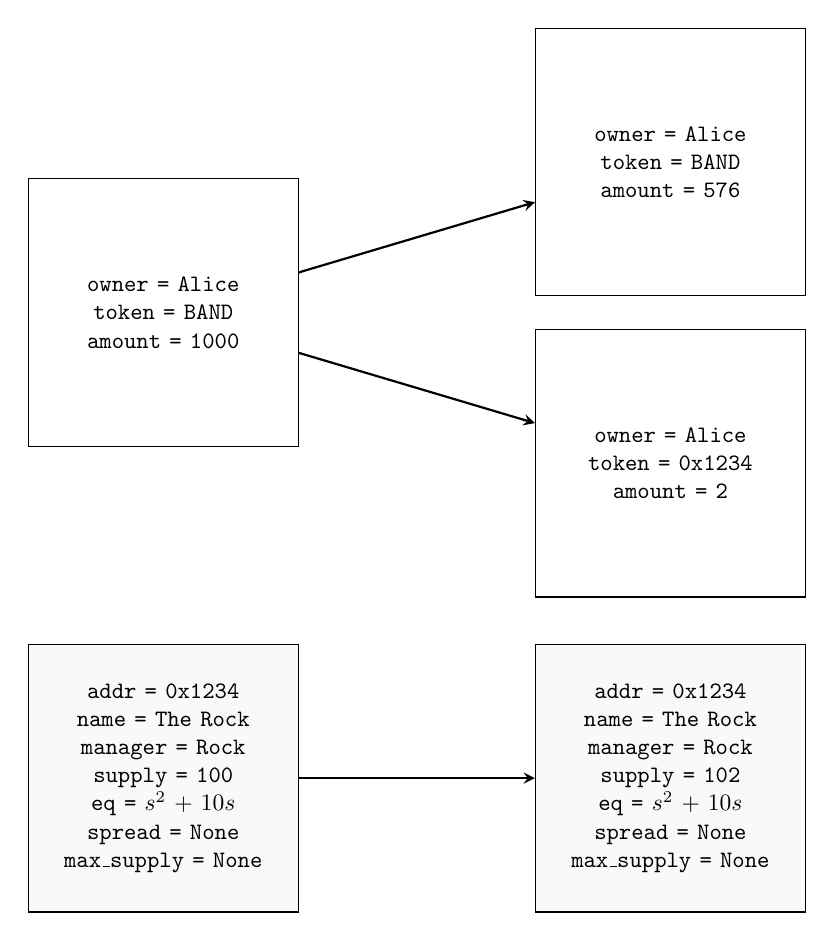
\begin{tikzpicture}
\node (alice-band-in) [utxo] {
    owner = Alice \\
    token = BAND \\
    amount = 1000
};

\node (rock-before) [contract,below=2.5cm of alice-band-in] {
    addr = 0x1234 \\
    name = The Rock \\
    manager = Rock \\
    supply = 100 \\
    eq = $s^2 + 10s$ \\
    spread = None \\
    max\_supply = None
};

\node (alice-band-out) [utxo, above right=-1.5cm and 3cm of alice-band-in] {
    owner = Alice \\
    token = BAND \\
    amount = 576
};

\node (alice-rock-out) [utxo, below right=-1.5cm and 3cm of alice-band-in] {
    owner = Alice \\
    token = 0x1234 \\
    amount = 2
};

\node (rock-after) [contract,right=3cm of rock-before] {
    addr = 0x1234 \\
    name = The Rock \\
    manager = Rock \\
    supply = 102 \\
    eq = $s^2 + 10s$ \\
    spread = None \\
    max\_supply = None
};

\draw [arrow] (alice-band-in) -- (alice-band-out);
\draw [arrow] (alice-band-in) -- (alice-rock-out);
\draw [arrow] (rock-before) -- (rock-after);
\end{tikzpicture}
\caption{An action of purchasing 2 ``The Rock'' token by Alice when the current supply is 100. Alice's BAND UTXO gets destroyed and she gets 2 new UTXO, one for BAND ``change'' and one for ``The Rock'' token. The community token contract's total supply value increases by 2.}
\label{fig:purchase-community-token}
\end{figure}

\subsection{Product Token} \label{sec:product-token}
Product Tokens are on-chain indivisible tokens that represent digital assets or digital vouchers that can be claimed for specific real-world products and services as set by Community Manager. For example, a musician may issue Concert Ticket Tokens that represent the right to claim a specific concert ticket. A celebrity can similarly issue digital collectible as Product Token with extremely limited supply.

Product Tokens can only be created by Community Manager who can customize parameters such as price, quantity, expiry date, sellability, etc. Price can either be fixed or can be issued with continuous bonding curve so dynamic demand and supply can dictate price. In the future, price can also be determined through auction for rare items.

There are benefits of issuing products through a blockchain-based Product Tokens for both Community Manager and mass consumers:

\paragraph{Extra Revenue} Community Manager can create extra revenue by selling new type of digital products such as scarce digital collectible (e.g. sticker packs, exclusive poster, animated gifs).

\paragraph{Dynamic Pricing} Community Manager can maximize revenue for certain non-rivalrous goods by creating a dynamic price based on continuous bonding curve which leads to optimal price discovery.

\paragraph{Liquidity Premium} Product Tokens can be easily traded in a global secondary market as there is a liquid market to trade products for specific community.

\paragraph{Transparency} There is full transparency when selling Product Tokens in terms of price, quantity and the mechanism of which product tokens are sold. For example, limited ticket concert can be sold to lottery winners using an open-source algorithm that determines winners so there is no way insider can cheat. It is also impossible to create counterfeit items.

\paragraph{Beneficiary Model} Beneficiary of product's revenue can be specified and automatically enforced through Product Token Contract. For example, 1\% of revenue will go toward charity can be strictly enforced since the contract issuance.

\subsubsection{Issuance}
Similar to Community Token, Community Manager can create Product Token with a specified bonding curve. This curve allows the price of Product Token, denominated in Community Token, to change based on the current total supply. Additionally, Product Token Contract contains three more parameters.

\paragraph{Bonded} The token creator can decide if the Product Token is ``bonded''. That is, whether a user can sell the tokens back to the Product Token Contract at the bonding curve price, potentially with price spread.

\paragraph{Sellable} The token creator can decide if the product token can be bought or sold in BAND's on-chain marketplace.

\paragraph{Transferable} The token creator can also decide if the token ownership can be transferred to other members of the community.

There is one distinction to note: if the Product Token is not bonded, token creator is able to additionally include the pricing variables such as $P_{\mathit{BNDUSD}}$, and the extra variable $\alpha$ representing the conversion rate of how many BAND is worth 1 Community Token, which is computed using the median of medians algorithm~\cite{wiki:mom}, similar to how pricing variables are calculated (See~\cref{sec:on-chain-px-oracle}) to prevent price manipulation. Formally, the value-supply grammar is extended with the following two constructs:

\begin{align*}
V \leftarrow
\begin{cases}
V & \text{Community Token price structure} \\
p & \text{A pricing variable $P_{\mathit{BNDUSD}}, P_{EURUSD}, ...$} \\
\alpha & \text{conversion rate of Community Token - BAND}
\end{cases}
\end{align*}

For instance, if the creator decides a concert ticket should be priced 1 dollar for the first ticket, 2 dollars for the second ticket, and so on. The pricing function would be $P(s)=  \alpha \times P_{\mathit{BNDUSD}} \times(s+0.5)$. The equation to put into the contract would be the anti-derivative of this equation with respect to s, which is $V(s) = \alpha \times P_{\mathit{BNDUSD}} \times 0.5 \times (s^2+s)$. If a person buys 3 tokens moving from total supply = 3 to 6, he must pay $V(6)-V(3) = 15 \alpha \cdot P_{\mathit{BNDUSD}} $ community token, which is approximately 15 dollars.

This scheme of value-supply equation gives the Community Manager a wide range of possibilities in defining the bonding curve of Product Token. The table below gives a few interesting examples.

\begin{adjustwidth}{-1.74cm}{}
\begin{center}
\begin{tabular}{ >{\footnotesize}c | c | c | c }
Price Model & $P(s)$ & $V(s)$ & {\footnotesize Can be Bonded} \\ \hline
Fixed price at 1 Comm token & $1$ & $s$ & Yes \\ \hdashline
Fixed price at 1 BAND token & $P_{\mathit{BNDUSD}}$ & $s \cdot P_{\mathit{BNDUSD}}  $ & No \\ \hdashline
Fixed price at 1 USD & $\alpha \cdot P_{\mathit{BNDUSD}}$ & $\alpha s \cdot P_{\mathit{BNDUSD}}  $  & No \\   \hdashline
Linearly increase in terms of BAND & $2s \cdot P_{\mathit{BNDUSD}} \times s$ & $s^2 \cdot P_{\mathit{BNDUSD}} $ & No \\   \hdashline
Exponentially increase in terms of Comm token & $3s^2$ & $ s^3$ & Yes \\  \hdashline
\begin{tabular}{@{}c@{}}Exponentially increase in terms of Comm token \\ with initial price of 10 USD\end{tabular} &
$3s^2 +10 \alpha \cdot  P_{\mathit{BNDUSD}}$ &
 $ s^3 + 10 \alpha s  \cdot P_{\mathit{BNDUSD}} $ & No

\end{tabular}
\end{center}
\end{adjustwidth}

\subsubsection{Redemption}
Since Product Tokens represent the right to claim real-world products and services from Community Manager, it requires a secure and private way to transact data between on-chain ownership of Product Token and off-chain private data required to claim products and services. For example, customer A needs to send CD token to a community manager sink address on-chain while sending a full name and address along with a signed message to community manager off-chain.

To redeem Product Token, a customer broadcasts a {\tt SPEND} transaction that signs the Product Token with user's provided information and marks it ``spent''. As a result of this transaction, the customer receives a ``receipt'' output that can be used as evidence of the payout. The customer can also attach extra information, such as an encrypted physical address to the receipt. This information can be used as the evidence should any disagreement occur. The Community Manager receives the spent Product Token, and if the Product Token is bonded, Community Manager can send the token back to the Product Token Contract to receive revenue in terms of Community Token.

\begin{figure}[!h]
\centering
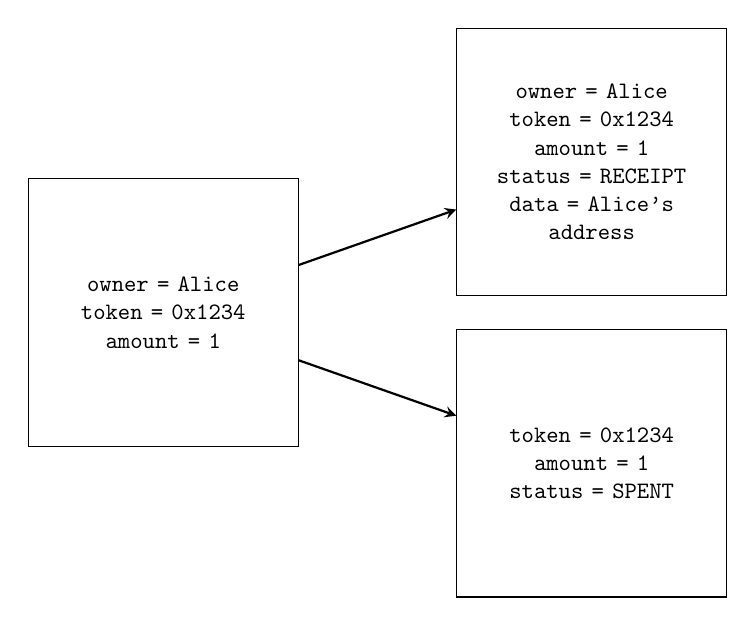
\begin{tikzpicture}[node distance=7cm]
\node (node1) [utxo] {
    owner = Alice \\
    token = 0x1234 \\
    amount = 1
};

\node (node2) [utxo, above right=-1.5cm and 2cm of node1] {
    owner = Alice \\
    token = 0x1234 \\
    amount = 1 \\
    status = RECEIPT \\
    data = Alice's address
};

\node (node3) [utxo, below right=-1.5cm and 2cm of node1] {
    token = 0x1234 \\
    amount = 1 \\
    status = SPENT \\
};
\draw [arrow] (node1) -- (node2);
\draw [arrow] (node1) -- (node3);
\end{tikzpicture}
\caption{An action of spending 1 Product Token by Alice. She is able to append her encrypted address to the receipt UTXO. Another UTXO is created for the Community Manager to sell it back for Community Token.}
\label{fig:utxo-stake}
\end{figure}

\subsubsection{Beneficiary}
Community Manager may wish to sell products and allocate a portion of revenue to a beneficiary or multiple beneficiaries. Since revenues are denominated in Community Token, a portion of divisible Community Token can be sent directly to a set of beneficiaries (addresses) specified in the contract. For example, 20\% of all revenues can be sent directly to Record Label Company and 0.5\% is sent to application owner who operates the application on top of the BAND Protocol.

In the future, when regulatory landscape allows ease of security offering, beneficiary model allows Community Manager to conduct their own fundraising and use beneficiary model to give part of future incomes to contributors. It allows young talented individuals to raise fund by themselves while community is able to invest in the potential of other individuals. For example, a writer may issue a new Community Token where he will sell his digital books and everyone who contribute in the initial stage will receive 50\% of all future revenue attached to the community.

At Product Token Contract creation, the Community Manager must specify addresses of beneficiaries with percentage of revenue ratio. Whenever a withdrawal request is processed, all pending Community Tokens (from buy/sell spread or for Product Token sellback by Community Manager) will be distributed according to the beneficiaries information.

\subsection{Marketplace} \label{sec:marketplace}
One of the main benefits of tokenized economy is the global liquidity. BAND Protocol establishes a standard marketplace contract for anyone to trustlessly buy and sell Product Tokens. Once there is a matched buyer and seller based on predefined price, Product Token and Community Token (payment) will be automatically swapped. Buyers are certain that seller has the real product while sellers are certain that buyers have the necessary money to purchase.

BAND blockchain supports atomic transfer of value. To do this, a user can convert his UTXO into an \emph{executable-UTXO} by broadcasting a {\tt MAKE\_TRADE} transaction. An executable UTXO is essentially an UTXO with the following added attributes:
\paragraph{Counter-Product} The product that can be traded with UTXO. This can be any other UTXO token types, including BAND, any Community Token, and any Product Token.
\paragraph{Equation} The equation specifies amount of counter-product required to transfer ownership of this UTXO. The amount is expressed in terms of an equation that can depends on any of the pricing variables and (prices) of any Community Token. \\

\begin{figure}[!h]
\centering
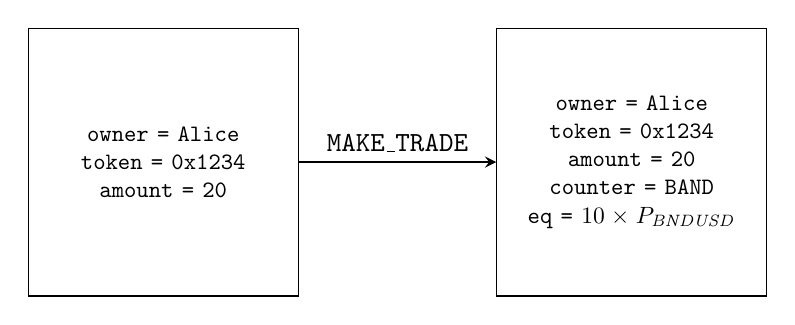
\begin{tikzpicture}[node distance=7cm]
\node (node1) [utxo] {
    owner = Alice \\
    token = 0x1234 \\
    amount = 20
};

\node (node2) [utxo, right of=node1] {
    owner = Alice \\
    token = 0x1234 \\
    amount = 20 \\
    counter = BAND \\
    eq = $10 \times P_{\mathit{BNDUSD}}$
};

\draw [arrow] (node1) -- node[anchor=south] {{\tt MAKE\_TRADE}} (node2);
\end{tikzpicture}
\caption{An action of converting 20 Community Token to be executable at price 10 USD}
\label{fig:utxo-stake}
\end{figure}

If another party agrees to trade, he can send his UTXO to execute with this executable-UTXO. If the amount condition is satisfied, the owner of both  UTXOs are swapped, on chain, in one blockchain operation. The UTXO owner, at any point, can decide to convert his executable-UTXO back to a normal UTXO, essentially cancel the offer to buy/sell products.

\begin{figure}[!h]
\centering
\begin{tikzpicture}[node distance=7cm]
\node (alice-utxo-in) [utxo] {
    owner = Alice \\
    token = 0x1234 \\
    amount = 20 \\
    counter = BAND \\
    eq = $10 \times P_{\mathit{BNDUSD}}$
};

\node (bob-utxo-out) [utxo, right=and 3cm of alice-band-in] {
    owner = Bob \\
    token = 0x1234 \\
    amount = 20 \\
};

\node (bob-utxo-in) [utxo,below=0.5cm of alice-band-in] {
    owner = Bob \\
    token = BAND \\
    amount = 30
};

\node (alice-utxo-out) [utxo, right=3cm of bob-utxo-in] {
    owner = Alice \\
    token = BAND \\
    amount = 30
};

\draw [arrow] (alice-utxo-in) -- (alice-utxo-out);
\draw [arrow] (bob-utxo-in) -- (bob-utxo-out);
\end{tikzpicture}
\caption{On-chain change of ownership of two UTXOs. The executable UTXO is priced at \$10. Note this this atomic swap can only take place when $P_{\mathit{BNDUSD}} = 3$.}
\end{figure}

Having this executable-UTXO paradigm, one can easily build a marketplace application that visualises easy-to-understand order book for each product-token pair on top of all UTXOs. For instances, if there exist three executable UTXOs of token {\tt 0x1234} to match with BAND and three different prices, the application can aggregate those values as asks of token {\tt 0x1234}. See~\cref{fig:marketplace-ex} as an example.

\begin{figure}[!h]
\centering
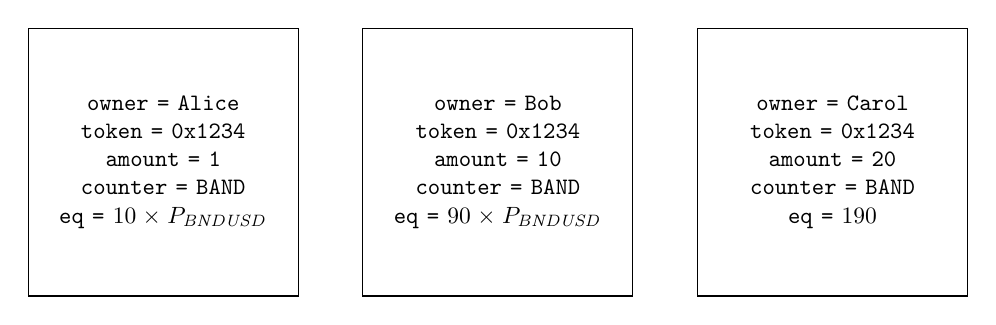
\begin{tikzpicture}[node distance=5cm]
\node (node1) [utxo]  {
    owner = Alice \\
    token = 0x1234 \\
    amount = 1 \\
    counter = BAND \\
    eq = $10 \times P_{\mathit{BNDUSD}}$
};

\node (node2) [utxo, right of=node1] {
    owner = Bob \\
    token = 0x1234 \\
    amount = 10 \\
    counter = BAND \\
    eq = $90 \times P_{\mathit{BNDUSD}}$
};

\node (node3) [utxo, right of=node2] {
    owner = Carol \\
    token = 0x1234 \\
    amount = 20 \\
    counter = BAND \\
    eq = $190$
};
\end{tikzpicture}
\begin{tabular}{ c | c | c | c | c }
No & Owner & Size & Price per token (BAND) & Price per token (USD) \\ \hline
1& Alice & 1 & 10 & 20 \\
2 & Carol & 20 & 9.5 & 19 \\
3 &Bob & 10 & 9 & 18 \\
\end{tabular}
\caption{There are three executable UTXOs for token {\tt 0x1234} priced at \$10, \$9, and 19 BAND. The figure shows an order book at the state where 1 BAND is priced at \$2.}
\label{fig:marketplace-ex}
\end{figure}
\subsection{Subscription Model} \label{sec:subscription-model}
BAND Protocol allows subscription business model in the new tokenized economy. A subscription model is generally when customer must pay a fixed amount of fee in a regular interval to have access to products or services. For example, a customer pays \$99 annually for Amazon Prime to get unlimited free shipping from Amazon. Another less straightforward example of subscription is annual membership fee. For example, Real Madrid Club Card costs \$170 annually which entitles card holder to receive a physical membership card, 10\% discount on all future purchases, access to newsletter, access to prize draw, etc.

In the BAND Protocol, Community Manager can create a similar subscription business model through a staking contract. Community members must stake a minimum amount of Community Token within certain period to earn the right to access certain products and services similar to a membership card. One notable difference is that community members must stake their tokens with a lock-up period to earn the right during the lock-up period. Once the lock-up period is over, they can either withdraw their token and forfeit future benefit or continue to stake their tokens to continue their benefit. This is different to general subscription model where customers must pay regularly. Note that if Community Managers wish to create a paying subscription model, they can create associated Product Token that has a validity for certain period of time (e.g. non-tradable Amazon Prime Product Token that entitles holder to receive free shipping benefit for one year.)

Community Manager can customize staking contract and benefit offered however they like. Tier system can be created where Community Manager defines minimum staking threshold in order to unlock certain benefits associated with each tier.

While subscription benefits can be customized depending on nature of the community, one standard benefit to subscription is the ability to receive discount on future purchases. Token holders are able to stake their tokens and receive Discount Token which is proportional to the amount of their staked token compared to total staked token in the system. Similar to how normal membership card entitles holder to receive discount on future purchases, token holders are loyal fan who will be rewarded through Discount Token. More detail is described in the subsequent section.

\subsubsection{Staking Contract}
A staking contract is created together with the creation of the Community Token. The Community Manager defines four parameters in the process:
\paragraph{Minimum Lockup Time} The minimum period before staked Community Token can be transformed back to unstaked Community Token.
\paragraph{Discount Interval} The interval where the revenue is aggregated and for which the Discount Token is valid. The Community Manager can choose one of the following choices: one week, two weeks, one month, two months, three months, and six months.
\paragraph{Ratio of Revenue as Discount} The ratio of revenue in the discount interval that will be distributed to users in form of Discount Token.
\paragraph{Discount Currency} The currency of Discount Token. This value can be Community Token, BAND token, or fiat currency. \\

At anytime community members are allowed to issue a staking transaction. As a result of the transaction, some amount of their Community Tokens will be transformed into a bonding note. After more than minimum lock-up time has passed, the owner of a bonding note may transform the note back to Community Token.

\begin{figure}[!h]
\centering
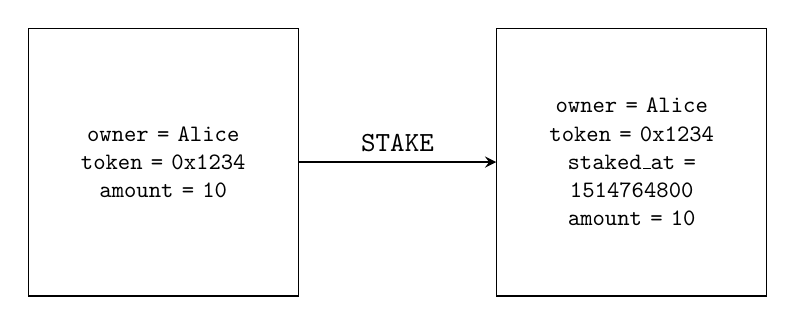
\begin{tikzpicture}[node distance=7cm]
\node (node1) [utxo] {
    owner = Alice \\
    token = 0x1234 \\
    amount = 10
};

\node (node2) [utxo, right of=node1] {
    owner = Alice \\
    token = 0x1234 \\
    staked\_at = 1514764800 \\
    amount = 10
};

\draw [arrow] (node1) -- node[anchor=south] {{\tt STAKE}} (node2);
\end{tikzpicture}
\caption{An action of staking 10 community token by Alice at epoch 1514764800 (Jan 1, 2018 12:00 AM)}
\label{fig:community-stake}
\end{figure}

\subsubsection{Discount Token}
At every discount interval, community member will be able to request Discount Tokens. The Discount Tokens will be determined by the ratio of the member's total lockup compared to the total lockup in the community and the total revenue of the community in that period. Discount Token will expire in the next discount interval, and a member will be able to request a new set of Discount Token for the next interval. The revenue is computed on chain using the following rules:

\begin{itemize}
\setlength\itemsep{0em}
\item For unbonded Product Token, any time Product Token is sold, the revenue is directly added to the community’s revenue pool, after being converted to discount currency at market rate.
\item For bonded product token, the revenue is computed at any time the Community Manager requests community Token withdrawal to all beneficiaries, after being converted to discount currency at market rate.
\end{itemize}

Formally, the total value of Discount Token that a user receives, in terms of Community Token, can be written the form of
\begin{align*}
D_{i} = \frac{C_{i}}{\Sigma C} \cdot \frac{\alpha_{0}}{\alpha_{t}} \cdot \mu \cdot (R_{\mathit{BONDED}} + R_{\mathit{UNBONDED}})
\end{align*}

Where $D_{i}$ is the total value Discount Token that user $i$ receives; $C_{i}$ is the total Community Token that user $i$ has staked over the discount interval period; $\alpha_{0}$ is the exchange rate of discount currency -- community token at the time the revenue is generated; $\alpha_{t}$ the same exchange rate at the time the Discount Token is used; $\mu$ is the Ratio of Revenue as Discount; $R_{\mathit{BONDED}}$ and $R_{\mathit{UNBONDED}}$ are the total revenue of bonded and unbonded product tokens respectively.

An unboned product token contract can be set to accept Discount Tokens as a payment. If that is the case, community members can choose to pay (partially or fully) via Discount Tokens that they possess. It is important to note that Discount Tokens are not transferable.

\begin{figure}[!h]
\centering
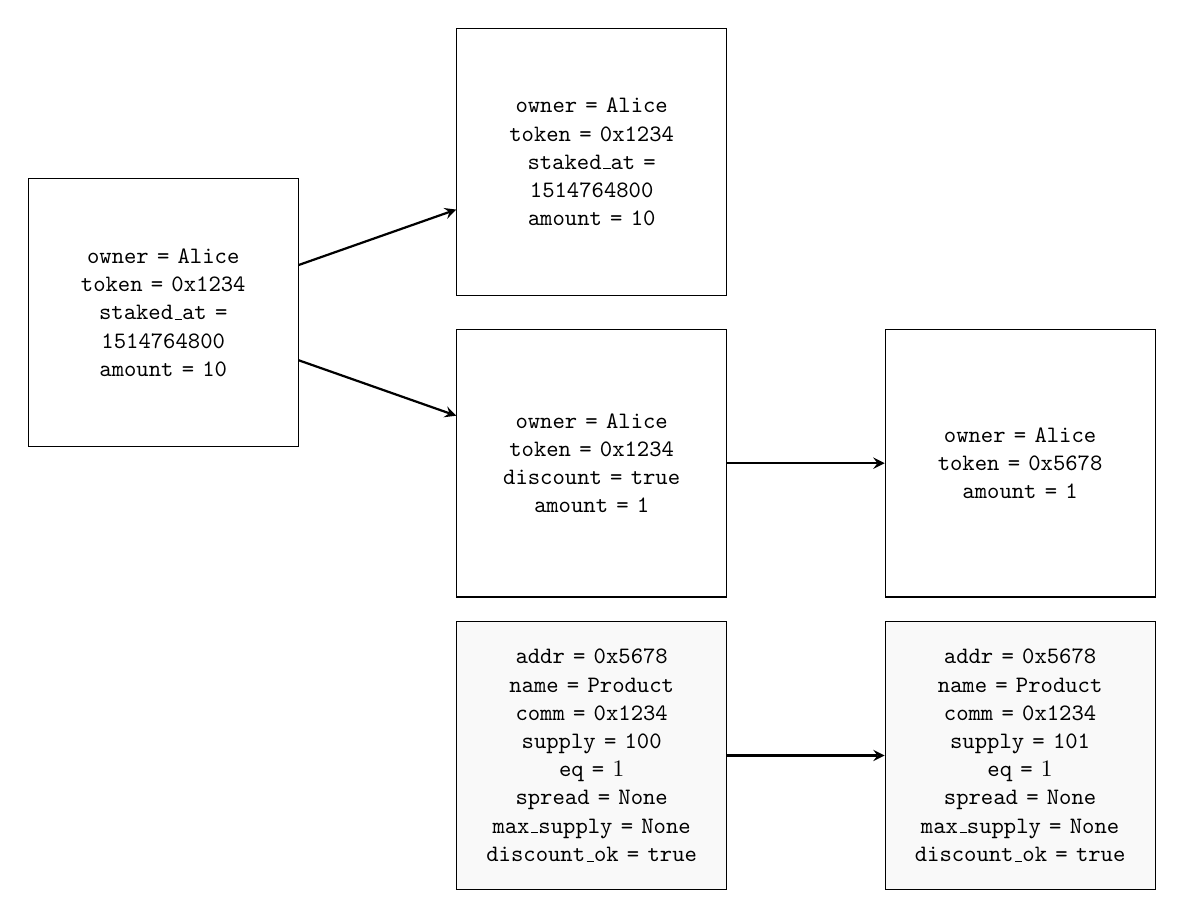
\begin{tikzpicture}
\node (alice-stake-in) [utxo] {
    owner = Alice \\
    token = 0x1234 \\
    staked\_at = 1514764800 \\
    amount = 10
};

\node (alice-stake-out) [utxo, above right=-1.5cm and 2cm of alice-stake-in] {
    owner = Alice \\
    token = 0x1234 \\
    staked\_at = 1514764800 \\
    amount = 10
};

\node (alice-discount-out) [utxo, below right=-1.5cm and 2cm of alice-stake-in] {
    owner = Alice \\
    token = 0x1234 \\
    discount = true \\
    amount = 1
};

\node (alice-product-out) [utxo, right=2cm of alice-discount-out] {
    owner = Alice \\
    token = 0x5678 \\
    amount = 1
};

\node (product-before) [contract,below=0.3cm of alice-discount-out] {
    addr = 0x5678 \\
    name = Product \\
    comm = 0x1234 \\
    supply = 100 \\
    eq = $1$ \\
    spread = None \\
    max\_supply = None \\
    discount\_ok = true
};

\node (product-after) [contract,right=2cm of product-before] {
    addr = 0x5678 \\
    name = Product \\
    comm = 0x1234 \\
    supply = 101 \\
    eq = $1$ \\
    spread = None \\
    max\_supply = None \\
    discount\_ok = true
};

\draw [arrow] (alice-stake-in) -- (alice-stake-out);
\draw [arrow] (alice-stake-in) -- (alice-discount-out);
\draw [arrow] (alice-discount-out) -- (alice-product-out);
\draw [arrow] (product-before) -- (product-after);
\end{tikzpicture}
\caption{An action of withdraw Discount Token from the community contract and spend it to buy a Product Token. Notice that the staked Community Token does not get spent at all.}
\label{fig:discount-full}
\end{figure}

\subsection{Attention Contracts} \label{sec:attention-contracts}
Attention curation market can be created in BAND tokenized economy. Since many Community Managers will gather large followers, many loyal followers will compete for the scarce attention of the Community Manager. BAND Protocol standardizes the way attention curation can occur in the protocol by allowing member of the communities to send Attention Tokens, a subclass of Product Token, and bond them to particular element such as post, comment, or any other elements as specified by the application. For example, an application built on top of BAND Protocol can easily create an Instagram-like application where followers can buy Attention Token and bond them to their comment similar to casting their vote. The application will then show top three comments so that Community Manager can see and interact with top comments who have the most amount of Attention Tokens bonded to them. The value of attention will depend on popularity of the Community Manager and amount of interaction received. Thus, Community Managers have an incentive to create an engaging community as it becomes a new monetization tool. Community Manager can finally monetize their loyal fan base and community.

On the protocol level, the manager creates an attention contract with arbitrary text information containing the purpose of this attention contract. Anyone can participate in this attention curation contract by sending Attention Product Token to the attention contract address with an arbitrary ``key'' information, likely their username on the application layer. The blockchain allows anyone to query the top keys with largest amount of contribution. This way the data is kept transparently forever on chain. As an example, the Community Manager of an Instragram-like website may create an attention contract for each image post. Users can send their Community Tokens to this contract to ``like'' the image. The application can query the blockchain to know the top contributed people to this image and reward them accordingly. \Cref{fig:attention-flow} shows the flow of attention curation contract.

\begin{figure}[!h]
\centering
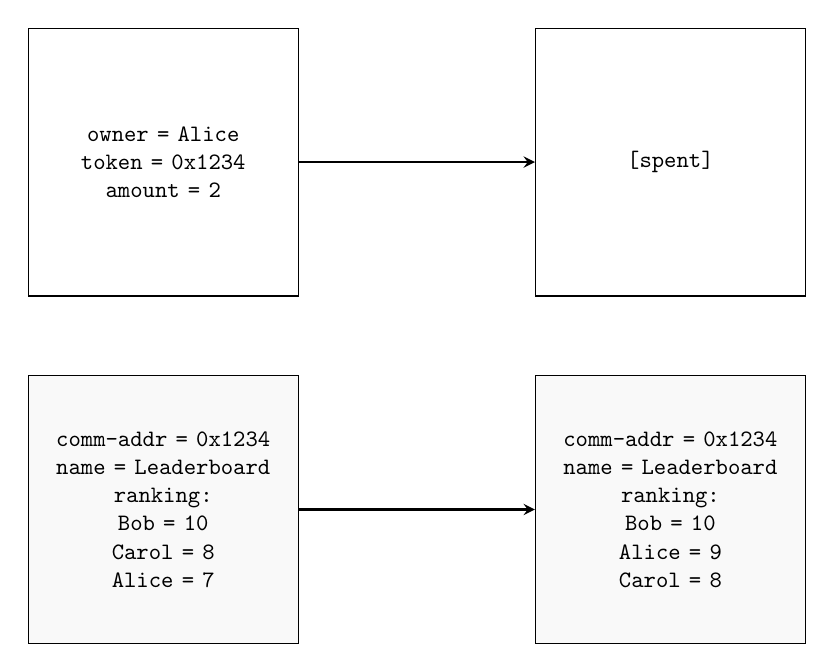
\begin{tikzpicture}
\node (alice-band-in) [utxo] {
    owner = Alice \\
    token = 0x1234 \\
    amount = 2
};

\node (attention-before) [contract,below=1cm of alice-band-in] {
    comm-addr = 0x1234 \\
    name = Leaderboard \\
    ranking:\\
    Bob = 10 \\
    Carol = 8 \\
    Alice = 7
};

\node (alice-band-out) [utxo, right=3cm of alice-band-in] {
    [spent]
};

\node (attention-after) [contract,right=3cm of attention-before] {
    comm-addr = 0x1234 \\
    name = Leaderboard \\
    ranking:\\
    Bob = 10 \\
    Alice = 9 \\
    Carol = 8
};

\draw [arrow] (alice-band-in) -- (alice-band-out);
\draw [arrow] (attention-before) -- (attention-after);
\end{tikzpicture}
\caption{An action of sending 2 Community Token from Alice to an attention contract too boost her rank in the leaderboard. Her Community Token gets spent in the process.}
\label{fig:attention-flow}
\end{figure}

\subsection{Service API Contracts} \label{sec:permission-contracts}
A service API contract is a standalone contract issued by Community Manager. It describes a condition that a community member must satisfy in order to use a particular service in the community. For example, a musician group community manager may define a service API contract for accessing free music streaming as ``the user must have at least 10 music streaming Product Token or stake at least 100 Community Token''. Formally a service contract contains one or more of the following conditions joint with binary logical operators.

\begin{itemize}
\setlength\itemsep{0em}
\item The user must own at least $x$ amount of Product Token at address $addr$
\item The user must has at least $x$ amount of Community Token at address $addr$ on stake
\end{itemize}

Once the service API is created, anyone can query the blockchain asking if a particular user is entitled to a particular service based on the service contract. Service APIs add more transparency to the network since anyone can check if they satisfy a condition that allows them to use a service.

\pagebreak

\section{Client Layer}
One of the main roadblocks of cryptocurrency's mass adoption is usability. Non-technical users struggle to understand and interact directly with blockchain layer and public-private keys. User-friendly applications are necessary to bring benefit of BAND Protocol to general mass consumers even if they are not familiar with its technical aspect. Campbase will be the first consumer application developed in conjunction with BAND Protocol. Since BAND Protocol is an open, permissionless blockchain protocol, anyone can build client application on top of the protocol.

\subsection{Campbase}
Campbase is the first tokenized marketplace centered around celebrities in the creative industry. In particular, Campbase targets individuals in the following creative economy: music, art, film, publishing, and sport. As individuals in the creative industry tend to gather loyal followers, they are apt to be among the early adopter of the platform as they have a new way to connect and monetize their large fan base.

\subsection{Problem Definition}
Current creative industry is facing a monetization problem as it becomes increasingly harder for them to directly sell their original content. Publishers and content distributors are two big middlemen who take big cut of the profit created by individual. With the emergence of Internet technology, platform companies are bringing in huge revenue while original content providers or celebrities receive little share of the revenue. For example, musician receives less than one cent per play on Spotify which unsurprisingly leads to ongoing feud between streaming service and artists~\cite{taylorswiftspotify, jayzspotify}. Similarly, famous celebrities amass millions of followers on content platform such as Facebook, Instagram and Twitter but they receive tiny share of the advertising revenues from these content aggregating platforms. Facing such issue, many celebrities turn to advertising model where third party companies pay celebrities to advertise company's products. This practice leads to misleading information for consumers as those sponsored advertisements are not truly transparent and are often masked as an endorsement of the celebrities. For example, a recent dispute on social media exposed one social media celebrity who demanded a luxurious Dubin hotel to give her free accommodation in exchange for free exposure on Instagram to her 80,000 followers. This sparks debate around the moral and ethical implication of how celebrities use their fame to promote products inorganically and mislead their followers~\cite{dublinban, hotelban}. There should be a new way for artists and content provider to monetize their products and services. Most importantly celebrities should be able monetize their own fan base while keeping incentives aligned with their followers.


\subsection{Solution}
Campbase will be the first decentralized platform for celebrities in creative industry to monetize their followers. As Taylor Swift aptly said: “music is art, and art is important and rare. Important, rare things are valuable. Valuable things should be paid for.”~\cite{taylorswiftspotify}

Campbase allows celebrities to monetize their rare attention and sell their products on a blockchain-based social platform. In particular, Campbase has five main features for each community which are described in the subsequent sections:
\begin{itemize}
\setlength\itemsep{0em}
\item Story Feed
\item Fan Feed
\item Event
\item Subscription
\item Store
\end{itemize}

%(pictures of ui/ux)

Celebrities will use Campbase to issue their unique Community Token which links to the overall value of their community. Community Token will be used as a primary currency in the community, as a stake to subscribe to discounts and other benefits customized by Community Manager and as a main token to buy attention and curate the community. As more consumers follow the community and stake their Community Tokens to receive discounts, they will be incentivized to spend those discounts and purchase more goods and services. In turn, more economic activities drive larger discount for loyal token holders. Positive feedback loop generates greater demand for followers to obtain Community Token and become part of loyal community. Both celebrities and followers can benefit from this tokenized economy and curation market.

\subsubsection{Story Feed}
Story Feed is the main content page curated by Community Manager. Community Manager can share text-based posts, images, or videos to their followers similar to typical social media platform. Followers can interact with their Community Manager by posting comments. Campbase creates attention curation market by allowing followers to vote on comments using Attention Token bought from the store with their Community Token. Most voted comments in each post will be shown on the feed so that Community Manager can easily interact with loyal followers. As Community Manager grows in popularity and more loyal followers demand his or her attention, the more Attention Token they are willing to pay and vote for their comments. This dynamic creates a new revenue stream for Community Managers. Since their attention is rare, their attention will become a new valuable in the tokenized economy.

\subsubsection{Fan Feed}
Fan Feed is the secondary content page curated by the community. Community members can post their own image, preferrably related to the community topic such as their pictures with Community Manager. They can similarly vote and interact with each other via comment section. Community Manager also has incentive to interact with the community through the Fan Feed to keep community more engaging. The more interaction is desired by community member, the more valuable the attention is.

\subsubsection{Event}
Community Manager in the creative industry is likely to hold multiple events such as concert, meet \& greet, autograph event, etc. Event tab will organize all relevant events held by Community Manager so that their followers can easily follow their schedule. Community Manager can also directly monetize their event by selling entrance ticket through the application.

\subsubsection{Subscription}
Subscription tab allows community manager to create their own subscription business model. Individuals in the creative industry produce many non-rivalrous goods which is suitable for a subscription model. For example, distributing book content to one consumer does not prevent another consumer to receive the same book content and the cost to providers is close to zero for each additional unit. This allows people to stake their Community Token and receives continuous benefits by being part of the loyal followers.

\subsubsection{Store}
Store has two main components: official store and P2P marketplace.

In the official store, consumers buy products and services in the form of Product Token directly from Community Manager. Community Managers can customize their product token and associated offers however they wish. Consumers can purchase product token using their Community Token directly in the official store.

In the P2P marketplace, consumers are able to list their product token and the price they want to sell at if the product token is tagged \textit{sellable} by Community Manager. Marketplace allows much better liquidity and transparency than traditional P2P market. For example, selling Concert Ticket Token on P2P marketplace ensures that the Concert Ticket Token is not a counterfeit while everyone in the community can easily browse through the marketplace, instead of on a third-party platform or in the physical world. It also allows Community Manager to profit from resellers as part of reseller's revenue can be configured to go directly to Community Manager’s beneficiary address.

\subsection{Community Manager}
After consulting with many creative publishers such as musicians, writers and artists, it is ostensibly clear that they need a new monetization channel for their content. Campbase will allow these creative publishers to create a new tokenized economy and bring in extra revenues.
\newline
\newline
Benefits to Community Manager include:
\begin{itemize}
\item Able to monetize their attention by curating their own community and respond to loyal fans who are willing to pay for their attention.
\item Able to directly monetize their traditional products and services on a unified social platform.
\item Able to offer new digital products such as rare digital collectibles related to the Community Manager. For example, a rare digital card collection, rare sticker pack which can be used to decorate customer’s picture on a feed, rare theme to be used inside the application, etc.
\item As more consumers participate in the tokenized economy, value of Community Token should rise in proportion to the total network value as consumers purchase more Community Token to receive continuous discounts and subscription benefits offered by the Community Manager.
\item Easy to bootstrap network effect and create loyal fan base for new individuals. Community Token incentivizes followers to curate the community and spread the attention of the community to wider audiences. Incentive is fully aligned between Community Manager and followers.
\end{itemize}

\subsection{Consumers}
Campbase similarly offer benefits to consumers compared to traditional platform as it becomes an all-in-one unified social media and marketplace. Traditionally, channels to follow their favorite celebrities are fragmented. Instagram provides picture feed, while event is often curated in a fragmented forum and official store is rarely formalized unless the celebrities are world-famous. Most simply lack the scale to operate their own store, website and social medias in one platform which makes it very difficult for consumers to follow their favorite celebrities. Campbase is an all-in-one platform for consumers to interact with their favorite celebrities while having an indirect incentive to promote the growth of the community.
\newline
\newline
Benefits to consumers include:
\begin{itemize}
\item Convenient access to follow their favorite celebrities.
\item New channel to interact directly with celebrities, which are very rare in traditional social media. This creates new connection as consumers are able to feel they are real and valuable part of the community. Community Tokens signify a loyal membership symbol.
\item Able to participate in celebrities' success. If consumers believe that the community will grow in the future, consumers can buy Community Token and subscribe to benefits and continuous discounts offered by the platform.
\item More transparent and liquid marketplace for official products. If consumers decide that they may not go to concert, they can easily list and sell through the P2P marketplace. Similarly, buyers can be sure they are getting the real product as Product Tokens are not forgeable.
\end{itemize}

\newpage

\section{Roadmap}

BAND Protocol has been conceived and been in active development since 2017. The following is our roadmap from ideation to our working product. Note that this is a targeted roadmap and may be subjected to change due to uncertainty in software development process.

\paragraph{Q3 - Q4 2017}
\begin{itemize}
\itemsep0em
\item Concept development
\item Research into crypto-primitives and technology
\item Market validation with real artists
\item Prototype different blockchain consensus protocol
\end{itemize}
\paragraph{Q1 2018}
\begin{itemize}
\itemsep0em
\item Draft whitepaper and go-to-market strategy
\item Draft yellowpaper
\item Begin product development
\end{itemize}
\paragraph{Q2 2018}
\begin{itemize}
\itemsep0em
\item Publish papers for peer-review
\item Launch our website
\item Launch our social media presence
\end{itemize}
\paragraph{Q3 2018}
\begin{itemize}
\itemsep0em
\item Launch testnet
\item Initiate bounty program
\item Initiate marketing campaign
\item Expand business partnership
\end{itemize}
\paragraph{Q4 2018}
\begin{itemize}
\itemsep0em
\item Launch first version of BAND Protocol with mainnet release
\item Launch Campbase with business partners and gather feedback
\item Publish official developer guidelines
\end{itemize}
\paragraph{2019}
\begin{itemize}
\itemsep0em
\item Integrate more product categories such as digital collectibles
\item Integrate stablecoin into ecosystem
\item Integrate auction, lottery and other pricing models
\item Integrate transparent voting mechanism
\item Refine user interface and overall experiences
\item Expand business partnership and onboard more celebrities to become global platform
\end{itemize}
\paragraph{2020}
\begin{itemize}
\itemsep0em
\item Expand to cover other industries such as consumer brand and general businesses
\item Work with regulatory body to create a framework to issue security tokens and allow individuals to hold crowdfunding (subject to shifting regulatory landscape)
\end{itemize}

\newpage

\bibliographystyle{unsrt}
\bibliography{paper}

\end{document}
